\section{Introduction}
\label{sec:intro}

\begin{figure*}[t]
  \centering
  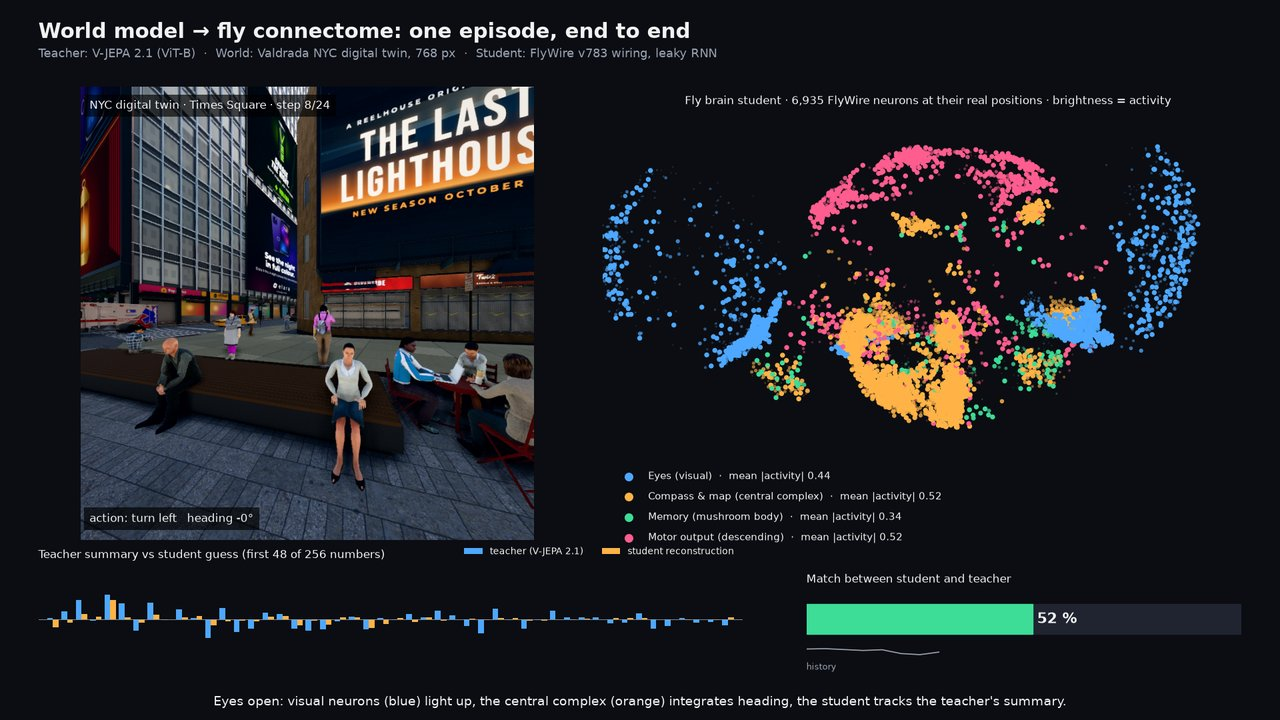
\includegraphics[width=0.495\linewidth]{fig/e2e_t07.jpg}\hfill
  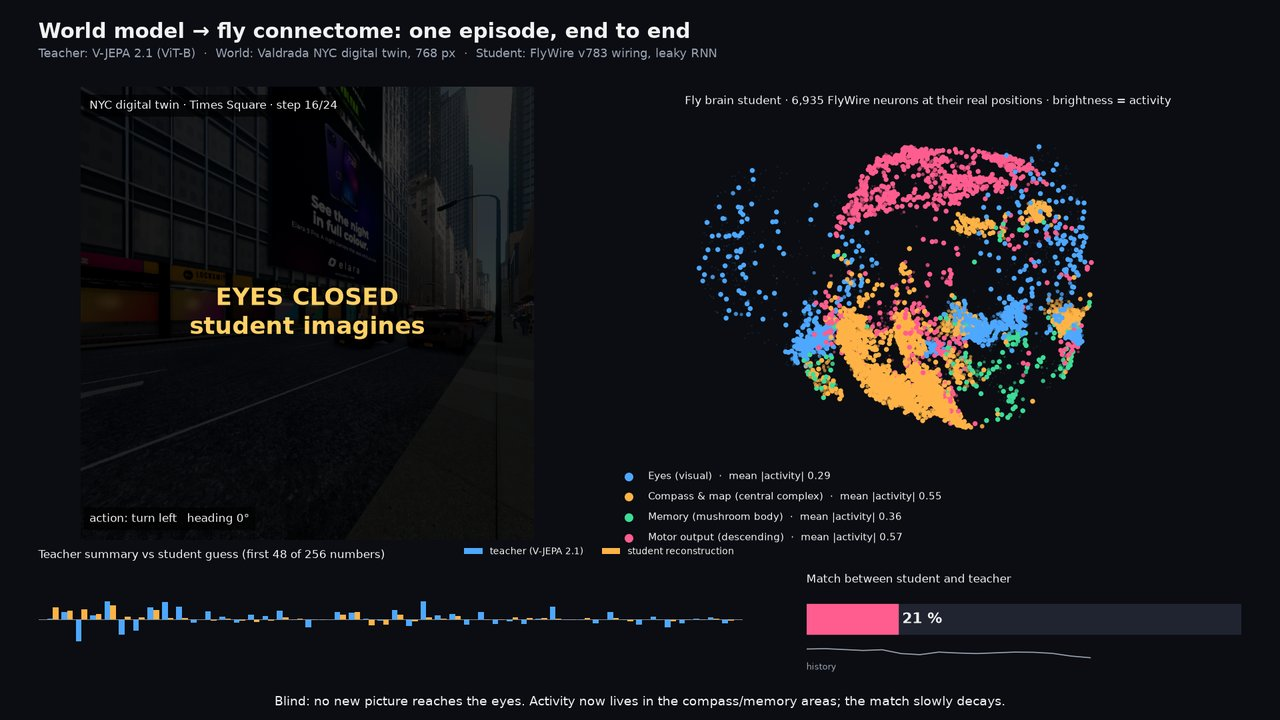
\includegraphics[width=0.495\linewidth]{fig/e2e_t15.jpg}
  \caption{\textbf{One episode, end to end, in the Manhattan twin.} Left: eyes open at step 8; the view the teacher
  encodes, the connectome student's activity drawn on the real \flywire soma positions (blue VIS, orange CX, green MB,
  pink OUT), the teacher's latent next to the student's reconstruction, and the match gauge. Right: eyes closed at step
  16; no new picture reaches the eyes, activity moves into the compass and memory populations, and the match decays
  slowly while the state keeps heading and position (\cref{sec:probes}). Full video in the supplement.}
  \label{fig:teaser}
\end{figure*}

\begin{figure*}[t]
  \centering
  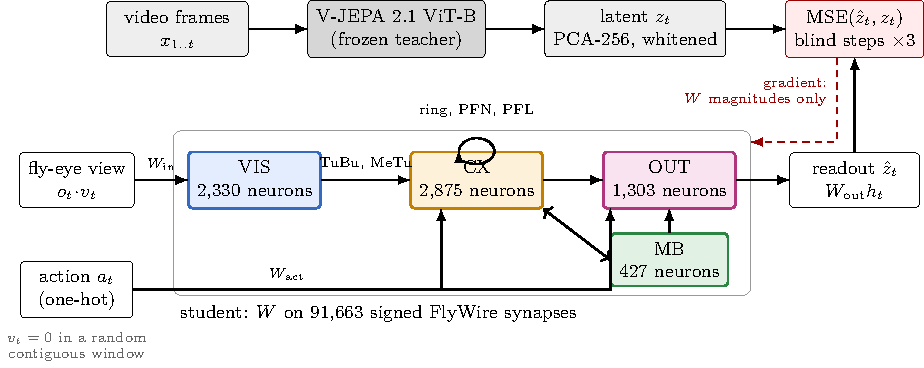
\includegraphics[width=\linewidth]{fig/pipeline.pdf}  % source: fig/src/pipeline.tex (build: fig/src/build.sh)
  \caption{\textbf{Pipeline.} A frozen \vjepa encoder turns each frame into a causal latent $z_t$. The student is a leaky
  rate network whose recurrence lives only on the signed synapses of four \flywire populations; training can rescale a
  synapse but never flip its sign, add one or remove one. The only training signal is next-latent prediction, with the
  view cut in a random window so the state must carry the latent on the action record alone. Heading, position and
  homing are read out of the trained state afterwards and were never supervised.}
  \label{fig:pipeline}
\end{figure*}

Ask a world model to imagine the next second of a video and it will do a reasonable job. Ask it what it imagines after
the lights go out, and the answer depends on what its recurrent core chose to remember. In most video world models that
core is a generic block, a GRU or a transformer layer, sized by compute and shaped only by the prediction
loss~\cite{ha2018world,hafner2023dreamerv3,assran2025vjepa2}. Biology solved the same problem differently. A fruit fly in
darkness holds its heading and a vector back to its start for many seconds using a few thousand central-complex
neurons, and the complete synapse-level wiring of that circuit is now
public~\cite{seelig2015neural,green2017neural,turnerevans2017angular,dorkenwald2024neuronal,schlegel2024whole}.

This paper puts the two together and asks one plain question: \emph{if a world model's recurrence is forced to be the
fly's wiring diagram, what does the wiring buy?} We distil \vjepa~\cite{assran2025vjepa2} into a leaky rate network of
6,935 \flywire neurons whose only recurrent weights sit on the 91,663 signed synapses of the real connectome
(\cref{fig:pipeline}). The student never sees the teacher's weights, only its latent through the loss, and is trained on
one objective: next-latent prediction under random blackouts of the visual input.

\paragraph{Why distillation, and why this kind}
Three alternatives were available and rejected. Training the connectome network directly on pixels would entangle the
wiring question with representation learning; fitting it to neural recordings, as prior connectome models
do~\cite{lappalainen2024connectome}, would answer a neuroscience question rather than a world-model question; and
distilling into a free architecture, as world-model compression does~\cite{hinton2015distilling,kasai2021t2r}, would
leave the wiring unconstrained. Latent-regression distillation from a frozen video encoder (the recipe of
DINO-WM~\cite{zhou2024dinowm} and JEPA world models~\cite{assran2025vjepa2}) is the one setting in which the student's
recurrence can be fixed to a biological graph while the target stays a strong, general, self-supervised representation.

\paragraph{What we find}
The answer has two halves, and we state both plainly. The wiring is \emph{not} a better predictor: against controls that
hold neuron count, edge count, region block structure, Dale's-law signs and parameter count fixed, the real connectome
beats its shuffled twins by about one percent of latent error, consistently, while a parameter-matched GRU is
\nGruBetterArena\,\% better. What the wiring buys is a \emph{path-integrating state} (\cref{fig:main}): during the blind
steps a ridge probe reads heading from the connectome state to \nConnArenaHd\degree\ median error and position to
$R^2$\,\nConnArenaPos, where the better-predicting GRU gives \nGruArenaHd\degree\ and \nGruArenaPos. The code survives 16
and 20 dark steps, reappears in a raycast twin of Manhattan, widens under a non-linear probe and persists under
continuous turn angles. Sparse random and block-shuffled wirings form it too, \nConnBlockGapArena\ to
\nConnBlockGapArenaDarkSixteen\degree\ worse: the exact synapse list is a small reproducible bonus, not the cause.

\begin{figure*}[t]
  \centering
  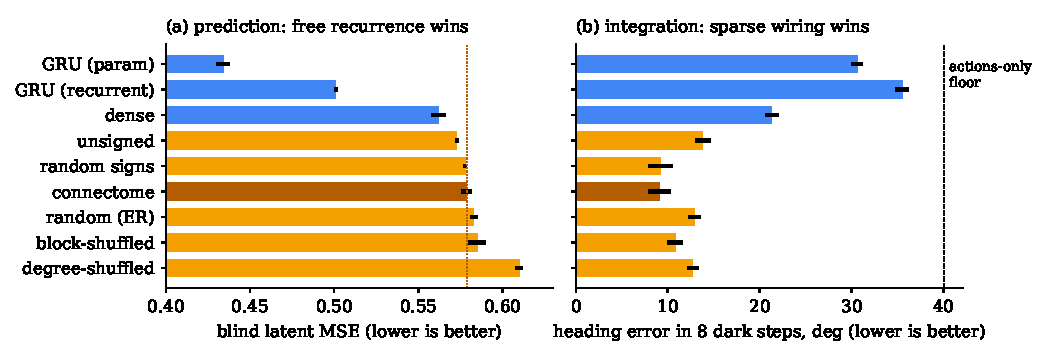
\includegraphics[width=\linewidth]{fig/ladder.pdf}
  \caption{\textbf{The wiring makes a worse predictor and a better integrator} (arena, mean\pm sd over 5 seeds).
  (a) Blind latent-prediction error: every free recurrence (blue) beats every fixed sparse graph (orange); the real
  connectome (dark) beats its shuffled twins by about one percent. (b) Median heading error decoded from the state
  during 8 dark steps: the ordering flips. Sparse signed graphs hold heading to about 10\degree, the GRUs to over
  30\degree, against a 40\degree\ floor for a linear readout of the actions alone.}
  \label{fig:main}
\end{figure*}

\paragraph{Contributions}
\begin{itemize}
  \item A distillation recipe that turns a video foundation model into a world model whose recurrence is a fixed,
        signed, biologically sourced sparse graph, with controls that separate wiring identity from density, degree
        sequence, region structure and sign structure (\cref{sec:method}).
  \item A single-versus-multiple-connectome study: $K$ copies of the brain coupled only through the 40,194 real
        commissural synapses, showing that neuron count is not the limiting resource (\cref{sec:multi}).
  \item The first demonstration, to our knowledge, that a connectome-wired latent predictor forms a linearly readable
        heading and position code in the dark that neither a GRU nor a transformer trained on the same objective forms,
        with information-ceiling, continuous-turn, feature-count and non-linearity controls (\cref{sec:probes}).
  \item A behavioural test of that code (blind homing, goal-vector navigation) with oracle, dead-reckoning and random
        controls, reported in full including the negative outcomes, plus real phone video as a third world
        (\cref{sec:behaviour,sec:realvid}).
  \item Two simulated environments, the real-video ingest pipeline, all code and checkpoints, released.
\end{itemize}
